\documentclass[a4paper, 11pt]{article}


\usepackage{geometry}
 \geometry{
 a4paper,
 total={170mm,257mm},
 left=20mm,
 top=20mm,
 }
\usepackage{listings}
\usepackage{graphicx}
\graphicspath{ {./images/} }
\usepackage[utf8]{inputenc}
\usepackage[T1]{fontenc}
\usepackage[polish]{babel}
\usepackage{listings}
\usepackage{natbib}
\usepackage{indentfirst}
\usepackage{hyperref}
\hypersetup{
    colorlinks=true,
    linkcolor=blue,
    filecolor=magenta,      
    urlcolor=cyan,
}
\lstdefinelanguage{scala}{
  morekeywords={abstract,case,catch,class,def,%
    do,else,extends,false,final,finally,%
    for,if,implicit,import,match,mixin,%
    new,null,object,override,package,%
    private,protected,requires,return,sealed,%
    super,this,throw,trait,true,try,%
    type,val,var,while,with,yield},
  otherkeywords={=>,<-,<\%,<:,>:,\#,@},
  sensitive=true,
  morecomment=[l]{//},
  morecomment=[n]{/*}{*/},
  morestring=[b]",
  morestring=[b]',
  morestring=[b]"""
}
\title{%
  Gilded Rose \\
  \large Projekt sklepu z przedmiotami - refactoring na przykładzie języka Scala}
\author{Dawid Bińkuś, 246793}
\begin{document}
\maketitle
\section{Wstęp}
\subsection{Źródła}
Przykład refactoryzacji w języku Scala został wykonany na podstawie projektu GildedRose.
\begin{itemize}
	\item Oryginalna treść projektu: \href{https://github.com/emilybache/GildedRose-Refactoring-Kata}{https://github.com/emilybache/GildedRose-Refactoring-Kata}
	\item Rozwiązanie zadania zaimplementowane w języku Scala \\\href{https://github.com/inql/zjp-assignment}{https://github.com/inql/zjp-assignment}
\end{itemize}
\subsection{Narzędzia wykorzystane do dokonania refactoryzacji kodu}
W celu rozwiązania zadania zostały wykorzystane następujące narzędzia:
\begin{itemize}
 \item Scalatest, wykorzystywany do implementacji testów jednostkowych: \href{http://www.scalatest.org/}{http://www.scalatest.org/}
 \item Scoverage, dodatek wykorzystywany do określenia pokrycia kodu przez testy:\\ \href{https://github.com/scoverage/sbt-scoverage}{https://github.com/scoverage/sbt-scoverage}
 \item Scapegoat, dodatek służący do określenia jakości kodu: \href{https://github.com/sksamuel/scapegoat}{https://github.com/sksamuel/scapegoat}
 \item SonarQube, narzędzie używane do analizy projektu wraz z dodatkiem \textit{sbt-sonar} wykorzystywanym do integracji w/w narzędzia z projektem: \href{https://github.com/mwz/sbt-sonar}{https://github.com/mwz/sbt-sonar}
\end{itemize}
\subsection{Omówienie kodu początkowego}
\subsubsection{Struktura klas}
Początkowa implementacja GildedRose składa się z dwóch klas:
\begin{itemize}
 \item \textbf{Item} - Klasa określająca strukturę przedmiotów w systemie - posiadaja ona informacje o nazwie przedmiotu, jakości oraz terminie w którym dany przedmiot ma być sprzedany.
 \item \textbf{GildedRose} - Klasa przechowująca logikę systemu GildedRose - zawiera tablicę przedmiotów obecnych w systemie. Dodatkowo, zawiera metodę umożliwiającą zaktualizować stan wszystkich przedmiotów.
\end{itemize}
\subsubsection{Omówienie logiki systemu GildedRose}
Zamysł logiki zaimplementowanej do systemu prezentuje się w sposób następujący:
\begin{enumerate}
 \item Sprawdzenie typu przedmiotu bazując na jego nazwie.
 \item Zmienienie jakości przedmiotu bazując na jego typie.
 \item Obniżenie terminu sprzedaży na przedmiocie.
\end{enumerate}
W zależności od typu przedmiotu mogą wystąpić dodatkowe efekty podczas aktualizacji danych, np. dla przedmiotu typu \textit{Aged Brie} jakość rośnie im dłużej jest magazynowany (tj. wartość terminu sprzedaży jest mniejsza niż zero), a właściwości przedmiotu typu \textit{Legendary} są stałe niezależnie od czasu spędzonego w systemie.
\subsubsection{Omówienie początkowej jakości kodu}
Początkowa logika systemu została napisany w sposób bardzo prosty a zarazem skomplikowany do zrozumienia. Cała logika opiera się na iteracji po poszczególnych przedmiotach w systemie a następnie zastosowaniu zmian zdefiniowanych w dokumentacji. Realnym problemem okazuje się sposób w jaki wykonywana jest ta czynność. Cała logika opiera się na skomplikowanej strukturze wyrażeń warunkowych, które rozgałęziają się i zagnieżdżają ze sobą co znacznie zwiększa złożoność implementacji.\\
Po początkowym skanowanie za pomocą narzędzia SonarQube kwestia jakości kodu została wyjaśniona:
\begin{figure}[!tbh]
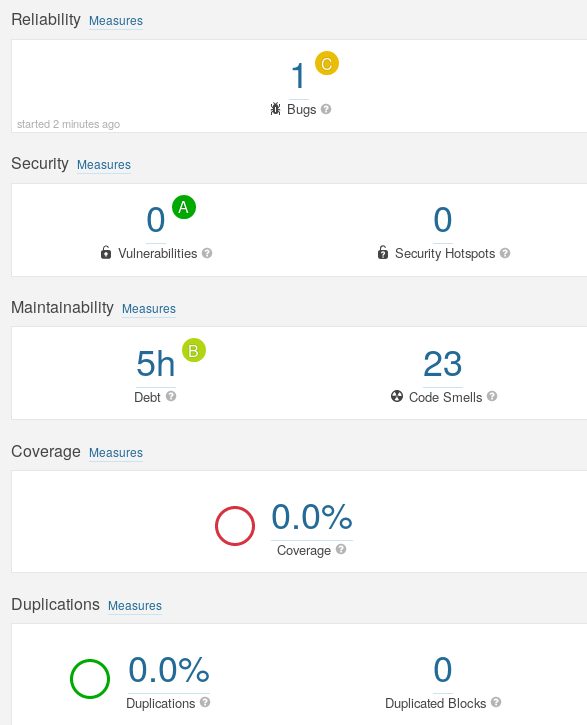
\includegraphics[width=8cm]{v01_ov}
\centering
\end{figure}\\
Bazując na rezultatach skanowania, znaczącym błędem mogącym prowadzić do nieprawidłowości było zerowanie wartości \textit{quality} produktu poprzez wykorzystanie danego wyrażenia:
\begin{lstlisting}[language=scala]
items(i).quality = items(i).quality - items(i).quality
\end{lstlisting}
Następnym obszarem wymagającym poprawy jest ogólnopojęta jakość kodu - SonarQube wykrył nieprawidłowości w postaci 23 \textit{Code Smells}. Dotyczyły one głównie braku odpowiedniego udokumentowania dla implementacji, zagnieżdżonych wyrażeń warunkowych oraz złożoności, utrudniającej zrozumienie instrukcji wykonywanych w programie.
\section{Omówienie procesu refactoryzacji}
W celu rozpoczęcia procesu refactoryzacji niezbędne było określenie jakie kolejne kroki należy podjąć by osiągnąć postawiony cel. Rozwój projektu podzieliłem na następujące etapy:
\begin{enumerate}
 \item Implementacja testów jednostkowych - zgodnie z zasadą \textbf{TDD}, chcemy mieć ciągłą kontrolę na poprawnością implementacji - w początkowej wersji projektu, testy nie były zaimplementowane.
 \item Uproszczenie głównej funkcji odpowiedzialnej za logikę projektu - by uczynić kod bardziej czytelnym i mniej skomplikowanym, należy całkowicie zmienić jego strukturę działania. Etap jest ten również przygotowaniem do kolejnej fazy.
 \item Implementacja nowej funkcjonalności - treść zadania wymaga dodania obsługi przedmiotów typu \textit{conjured} - po uproszczeniu logiki aplikacji zadanie to powinno być znacznie prostsze.
\end{enumerate}
\subsection{Implementacja testów}
Do implementacji testów wykorzystana została biblioteka \textit{Scalatest} - umożliwia ona pisanie testów w prosty sposób a wykonywane instrukcje powinny być zrozumiane również przez osobę nietechniczną. Dostarczona implementacja testów sprawdzała nieistotną w kontekście aplikacji funkcjonalność - możliwość zmiany przedmiotu po zaktualizowaniu wartości.
Początkowy kod prezentował się w sposób następujący:
\begin{lstlisting}[language=scala]
 class GildedRoseTest  extends FlatSpec with Matchers {
      it should "foo" in {
        var items = Array[Item](new Item("foo", 0, 0))
        val app = new GildedRose(items)
        app.updateQuality()
        (app.items(0).name) should equal ("fixme")
      }
}
\end{lstlisting}
W celu napisania nowej implementacji testów, pozbyto się całkowicie starej implementacji i zastosowano nową, wykorzystującą moduły \textit{FunSpec} oraz \textit{BeforeAndAfterEach}. Pierwszy z nich posłużył nam do ustruktoryzowania procedur testowych (testy napisane w ten sposób można podzielić według testowanego obszaru i konkretnego zachowania w myśl zasday \textbf{BDD}). Drugi zaś umożliwił zaimplementowanie metody \textit{beforeEach}, która przygotowywała stan systemu przed wykonaniem operacji określonych w teście.\\
Początkowa definicja testów prezentuje się w sposób następujący:
\begin{lstlisting}[language=scala]
class GildedRoseTest extends FunSpec with BeforeAndAfterEach {

  var regular, agedBrie, sulfuras, backstage: Item = _
  var gildedRose: GildedRose = _

  override def beforeEach(): Unit = {
    regular = new Item("regular", 7, 7)
    agedBrie = new Item("Aged Brie", 15, 15)
    sulfuras = new Item("Sulfuras, Hand of Ragnaros", 30,80)
    backstage = new Item("Backstage passes to a TAFKAL80ETC concert", 11, 9)

    gildedRose = new GildedRose(Array(regular,agedBrie,sulfuras,backstage))
  }
\end{lstlisting}
Po przygotowaniu systemu do wykonywania testów poprzez wstrzyknięcie mu niezbednych danych, należało przejść do implementacji zachowań do sprawdzenia.
Za pomocą instrukcji \textit{describe} określony został obszar testów (system GildedRose), następnie za pomocą instrukcji \textit{it} zdefiniowane zostały testy bazujące na określonych oczekiwanych zachowaniach systemu. Przykładowe testy prezentują się w sposób następujący:
\begin{lstlisting}[language=scala]
  describe("GildedRose"){

    it("should degrade item's quality by one when the day ends"){
      gildedRose.updateQuality()
      assertResult(6)(regular.quality)
    }

    it("should reduce item's sellIn by one then the day ends"){
      gildedRose.updateQuality()
      assertResult(6)(regular.sellIn)
    }

    it("should degrade item's quality twice when sellIn reached zero"){
      regular.sellIn = 0
      gildedRose.updateQuality()
      assertResult(5)(regular.quality)
    }

    it("should item's quality never reach zero"){
      regular.quality = 0
      gildedRose.updateQuality()
      assertResult(0)(regular.quality)
    }
\end{lstlisting}
Po przygotowaniu wszystkich testów, należało przystąpić do wykonania testowego uruchomienia. Wszystkie testy były uruchamiane zarówno lokalnie jak i z użyciem kontenera tworzonego na witrynie github.com - repozytorium projektu zostało skonfigurowane w taki sposób by każda aktualizacja wiązała się z wykonaniem całej sekwencji testowej.
\begin{figure}[!tbh]
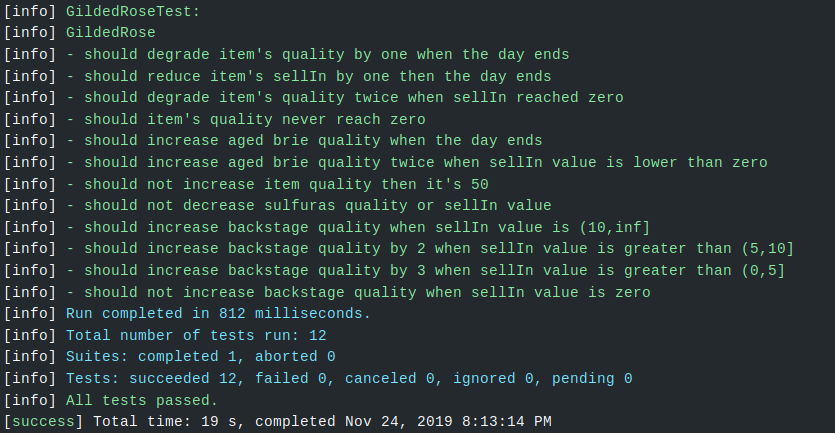
\includegraphics[width=8cm]{tests}
\centering
\end{figure}\\
Dzięki zaimplementowaniu testów jednostkowych, upewniliśmy się, że implementacja systemu mimo wątpliwej jakości, działa tak jak zakładaliśmy. Umożliwia to przejście do kolejnego etapu refactoryzacji.
Dodatkowo, osiągnięte zostało pokrycie kodu w postaci 100\% instrukcji zawartych w systemie GildedRose
\subsection{Upraszczanie kodu}
\subsection{Implementacja nowej funkcjonalności}
\section{Implementacja paradygmatu funkcyjnego do istniejącego kodu obiektowego}
\subsection{Wydzielenie logiki kodu}
\subsection{Funkcja jako wyrażenie}

\end{document}
